\documentclass{beamer}
\usepackage[T1]{fontenc}
\usepackage[utf8]{inputenc}
\usepackage{lmodern}
\usepackage[brazil]{babel}
\usepackage[labelformat=empty]{caption}
\usepackage{graphicx}
\usepackage{color}

\definecolor{beamer@blendedblue}{rgb}{0.5, 0.6, 0.4}
\definecolor{covered}{gray}{0.65}
\definecolor{filecolor}{rgb}{0, 0.3, 0.7}
\usetheme{Warsaw}
\title[NetSim: um simulador de redes simplificado.]{NetSim: um simulador de redes simplificado.}
\author{Carlos Eduardo Leão Elmadjian \and Renan Fichberg}
\date{11 de novembro de 2014}
\institute{Instituto de Matemática e Estatística da Universidade de São Paulo (IME-USP)}

\expandafter\def\expandafter\insertshorttitle\expandafter{%
\insertshorttitle\hfill%
\insertframenumber\,/\,\inserttotalframenumber}

\begin{document}

\begin{frame}
	\titlepage
\end{frame}

\begin{frame}
\begin{center}
	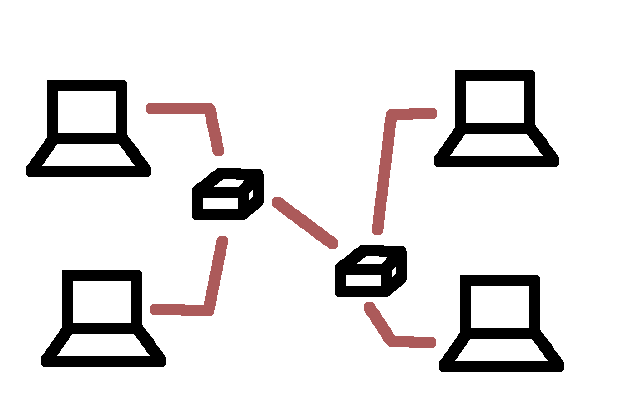
\includegraphics[scale=0.4]{simulator.png}
\end{center}
\end{frame}

\begin{frame}
	\frametitle{Conteúdo}
	\begin{itemize}
		\item O simulador: como funciona?
		\item Testes realizados com o simulador
		\item Dificuldades encontradas
	\end{itemize}
\end{frame}

\begin{frame}
	\frametitle{O simulador: como funciona?}
	\begin{itemize}
		\item Estrutura do NetSim
		\item Entradas
		\item Saídas
		\item As classes e as suas funções
	\end{itemize}
\end{frame}

\begin{frame}
	\frametitle{O simulador: como funciona?}
	\framesubtitle{Estrutura do NetSim}
	O NetSim é dividido em módulos. Isso foi pensado desta maneira pois, logo de inicio, 
	foi imaginado que haveriam muitas classes. Como o programa foi desenvolvido em Java, ao compilá-lo, 
	há um boom na quantidade de arquivos com o surgimento dos de extensão .class. 
	Com isto, para diminuir o caos no diretório que contém o código-fonte, há outros
	dois sub-diretórios:
	\begin{itemize}
		\item \textbf{/inputs} - Contém arquivos .txt com entradas para alimentar o simulador. É aqui que o usuário deve deixar suas entradas, \textbf{obrigatoriamente}.
		\item \textbf{/logs} - Contém arquivos .log com as saídas. As saídas são os pacotes capturados pelos \textit{Sniffers} definidos na entrada que alimentou o programa.
	\end{itemize}
\end{frame}

\begin{frame}
	\frametitle{O simulador: como funciona?}
	\begin{itemize}
		\item \textcolor{covered}{Estrutura do NetSim}
		\item Entradas
		\item Saídas
		\item As classes e as suas funções
	\end{itemize}
\end{frame}

\begin{frame}
	\frametitle{O simulador: como funciona?}
	\framesubtitle{Entradas}
	Há no total apenas \textbf{12} tipos de entrada esperadas pelo programa. São elas:
	\begin{itemize}
		\item Entrada para criação de computadores (\textit{hosts})
		\item Entrada para criação de roteadores (\textit{routers})
		\item Entrada para criação de enlaces do tipo duplex-link
		\item Entrada para configuração dos \textit{hosts} com relação aos endereços de IP do próprio computador, do roteador padrão e do servidor DNS
	\end{itemize}
\end{frame}

\begin{frame}
	\frametitle{O simulador: como funciona?}
	\framesubtitle{Entradas}
	\begin{itemize}
		\item Entrada para configuração dos \textit{routers} com relação às portas e aos endereços de IP
		\item Entrada para a configuração dos \textit{routers} com relação às rotas
		\item Entrada para a configuração dos \textit{routers} com relação aos seus dados de \textit{performance}
		\item Entrada para a configuração dos agentes da camada de aplicação: declaração do agente e da sua natureza 
	\end{itemize}
\end{frame}

\begin{frame}
	\frametitle{O simulador: como funciona?}
	\framesubtitle{Entradas}
	\begin{itemize}
		\item Entrada para a configuração dos agentes da camada de aplicação: associação do agente declarado a um \textit{host}
		\item Entrada para a configuração dos agentes da camada de aplicação: declaração dos \textit{sniffers}
		\item Entrada para a configuração dos agentes da camada de aplicação: locais da rede onde os \textit{sniffers} agirão.
		\item Entrada para a Configuração das comunicações entre os agentes.
	\end{itemize}
\end{frame}

\begin{frame}
	\frametitle{O simulador: como funciona?}
	\begin{itemize}
		\item \textcolor{covered}{Estrutura do NetSim}
		\item \textcolor{covered}{Entradas}
		\item Saídas
		\item As classes e as suas funções
	\end{itemize}
\end{frame}

\begin{frame}
	\frametitle{O simulador: como funciona?}
	\framesubtitle{Saídas}
	As saídas, como já mencionado anteriormente, são os resultados das capturas dos pacotes pelo \textit{sniffers}, e estas
	ficam armazenadas por default no sub-diretório de logs. Cada \textit{sniffer} tem seu próprio log, cujo o nome do arquivo tem o formato
	\textbf{nome\_do\_sniffer.log}. Este é o comportamento do programa para caso o usuário não passe uma saída da sua escolha. 
\end{frame}

\begin{frame}
	\frametitle{O simulador: como funciona?}
	\framesubtitle{Saídas}
	O formato da saída é o seguinte:
	\begin{itemize}
		\item Identificador do pacote
		\item Instante de tempo em que o pacote foi visto (a partir da execução do programa)
		\item Identificador do \textit{sniffer}
		\item Informações da camada de rede (IP):
		\begin{itemize}
			\item IP de origem
			\item IP de destino
			\item Identificação do protocolo da camada acima
			\item Tamanho cabeçalho IP + tamanho das camadas superiores
			\item TTL
		\end{itemize}
	\end{itemize}
\end{frame}

\begin{frame}
	\frametitle{O simulador: como funciona?}
	\framesubtitle{Saídas}
	\begin{itemize}
		\item Informações da camada de transporte (se for TCP):
		\begin{itemize}
			\item Porta origem
			\item Porta destino
			\item Tamanho cabeçalho TCP + tamanho da camada superior
			\item Número de Seqüência
			\item Número de Reconhecimento
			\item Bit ACK
			\item Bit FIN
			\item Bit SYN
		\end{itemize}
		\item Informações da camada de transporte (se for UDP):
		\begin{itemize}
			\item Porta origem
			\item Porta destino
			\item Tamanho cabeçalho UDP + tamanho da camada superior
		\end{itemize}
	\end{itemize}
\end{frame}

\begin{frame}
	\frametitle{O simulador: como funciona?}
	\framesubtitle{Saídas}
	\begin{itemize}
		\item Informações da camada de aplicação (DNS/FTP/HTTP):
		\begin{itemize}
			\item Pergunta ou resposta contida no pacote.
		\end{itemize}
	\end{itemize}
	Ainda, além das informações estarem presentes no log, a cada captura os resultados daquele \textit{sniffer}
	são imprimidos no \textit{prompt} em tempo de execução.
\end{frame}

\begin{frame}
	\frametitle{O simulador: como funciona?}
	\begin{itemize}
		\item \textcolor{covered}{Estrutura do NetSim}
		\item \textcolor{covered}{Entradas}
		\item \textcolor{covered}{Saídas}
		\item As classes e as suas funções
	\end{itemize}
\end{frame}

\end{document}